% ЕМТ 2024, IX клас — точен LaTeX препис от официалните файлове в Klasirane.com.
% Условия: https://klasirane.com/api/competitions/EMT/All/2024/9%20%D0%BA%D0%BB/probs
% SHA-256 (условия): 191a44a780109f63d252ad1b772bbfd596ed67564f8dc51f8af84ef98835b35c
% Решения: https://klasirane.com/api/competitions/EMT/All/2024/9%20%D0%BA%D0%BB/sol
% SHA-256 (решения): 682a8492b35693b53c3f7ffe9cc50af5ca4b38003fa137fec2444d216249672b
% Точковите оценки, правописът, формулировките и видимите печатни особености са запазени от източника.
% И двата PDF файла съдържат сканирани страници; видимите страници са проверени пряко.
% Фигурата към решение 9.2 е изрязана без прерисуване от сканираната страница на официалното решение.

Задача 9.1. Да се реши в реални числа системата
$$
\begin{cases}
\dfrac1x+\dfrac1y=2,\\
x^2y+xy^2=2.
\end{cases}
$$

Решение. Полагаме $p=x+y$, $q=xy$, с което системата добива вида
$$
\begin{cases}
\dfrac pq=2,\\
pq=2.
\end{cases}
$$
Да отбележим, че $x$ и $y$ са корени на квадратното уравнение $t^2-pt+q=0$. Умножавайки двете уравнения от последната система, получаваме $p^2=4$, следователно $p\in\{\pm2\}$. При $p=2$ имаме $q=1$ и значи $x,y$ са корени на уравнението $t^2-2t+1=0$, т. е. $x=y=1$. При $p=-2$ и $q=-1$ квадратното уравнение е $t^2+2t-1=0$ и има корени $\{x,y\}=\{-1+\sqrt2,-1-\sqrt2\}$. Окончателно всички решения на системата са
$$
(x;y)=(1;1),\ (-1+\sqrt2;-1-\sqrt2),\ (-1-\sqrt2;-1+\sqrt2).
$$

Оценяване. (6 точки) 2 т. за полагането; 2 т. за случая $p=2$; 2 т. за случая $p=-2$.

Задача 9.2. Даден е остроъгълен разностранен триъгълник $ABC$ с височини $AE$ и $BD$. Върху правата $AC$ са взети точки $G$ и $M$, такива че $AE=AG=AM$ и $C$, $G$, $A$, $M$ лежат в този ред. Върху правата $BC$ са взети точки $F$ и $L$, такива че $BD=BF=BL$ и $C$, $F$, $B$, $L$ лежат в този ред. Нека $P$ е средата на $DE$. Да се докаже, че перпендикулярът от $P$ към $AB$ и правите $EM$ и $DL$ се пресичат в една точка.

Решение.

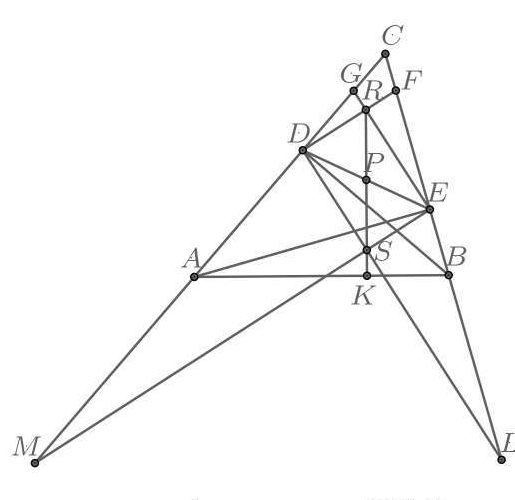
\includegraphics[max width=0.46\textwidth, alt={Официалната фигура към решение 9.2 с триъгълника ABC и точките D, E, F, G, K, L, M, P, R и S}, center]{assets/9-2-geometry.png}

Използваме стандартните означения $\alpha$, $\beta$, $\gamma$ за ъглите на $ABC$. Нека означим $R=DF\cap GE$ и $S=ME\cap DL$. Можем да намерим, че $\angle DEG=\angle AEG-\angle AED=45+\dfrac\gamma2-(90-\alpha)=\alpha+\dfrac\gamma2-45$ и $\angle EDF=\beta+\dfrac\gamma2-45$, откъдето $\angle DRE=90$. С подобно изразяване намираме $\angle SDE=\angle SDB+\angle BDE=45-\dfrac\gamma2+90-\beta=135-\beta-\dfrac\gamma2=\angle DEG$, $\angle SED=135-\alpha-\dfrac\gamma2=\angle BDF$ и $\angle DSE=90$. Оттук лесно получаваме, че $\angle SDR=\angle SER=90$, следователно $DRES$ е правоъгълник и значи $P$ лежи на отсечката $RS$.

Накрая ако означим с $K$ пресечната точка на $AB$ и $RS$, то с изразяване на ъгли в четириъгълника $BKRE$ намираме
$$
\angle KRE+\angle REB+\angle EBK=135-\beta-\frac\gamma2+\left(45+\frac\gamma2+90\right)+\beta=270,
$$
следователно $\angle RKB=90$ и значи $RS\perp AB$. Тогава перпендикулярът от $P$ към $AB$ съвпада с правата $RS$, с което завършваме доказателството.

Оценяване. (6 точки) 1 т. за получаване на $\angle DRE=90^\circ$ или $\angle DSE=90^\circ$; 1 т. за обосновка на $\angle SDR=\angle SER=90^\circ$ и извод, че $DSER$ е правоъгълник; 1 т. за извод, че $P$ лежи на $RS$; 2 т. за доказване, че $RS\perp AB$; 1 т. за завършване. При липса на което и да е от горните се дава 1 т. за доказване, че $DGFE$ или $DELM$ е вписан четириъгълник.

Задача 9.3. Едно естествено число наричаме свободно от квадрати, ако не се дели на квадрата на никое просто число.

За естествено число $a$ разглеждаме числото $f(a)=a^{a+1}+1$. Докажете, че:

а) ако $a$ е четно, то $f(a)$ не е свободно от квадрати.

б) съществуват безбройно много нечетни $a$, за които $f(a)$ не е свободно от квадрати.

Решение. а) Нека $p$ е просто число, което дели $a+1$ (такова има, тъй като $a+1>1$). Понеже $a+1$ е нечетно, то можем да разложим
$$
a^{a+1}+1=(a+1)(a^a-a^{a-1}+\cdots-a+1).
$$
Сега е ясно, че $a^a-a^{a-1}+\cdots-a+1\equiv(-1)^a-(-1)^{a-1}+\cdots-(-1)+1\equiv a+1\equiv0\pmod p$ и значи $p^2\mid a^{a+1}+1$.

б) Първи метод. Да забележим, че ако $p\mid a^{a+1}+1=\left(a^{\frac{a+1}{2}}\right)^2+1$, то $p\equiv1\pmod4$. При фиксиран избор на такова $p$ ще построим нечетно $a$, за което $p^2\mid a^{a+1}+1$. Понеже простите числа от вида $4k+1$ са безбройно много и всяко число $a^{a+1}+1$ има краен брой прости делители, това е достатъчно, за да докажем твърдението.

И така, нека $p\equiv1\pmod4$ е фиксирано. Ако намерим $a$, за което $p^2\mid a^2+1$ и $a\equiv1\pmod4$, то $a$ ще е нечетно и $p^2\mid a^2+1\mid(a^2)^{\frac{a+1}{2}}+1=a^{a+1}+1$. За целта първо намираме естествено число $x$, за което $p\mid x^2+1$ (например $x=\left(\dfrac{p-1}{2}\right)!$). След това разглеждаме числата
$$
x^2+1,\ (x+p)^2+1,\ (x+2p)^2+1,\ldots,\ (x+(p-1)p)^2+1, \tag{*}
$$
всяко от които се дели на $p$. Ако допуснем, че за някои $k,\ell\in\{0,1,2,\ldots,p-1\}$ с $k\neq\ell$ е изпълнено
$$
(x+kp)^2+1\equiv(x+\ell p)^2+1\pmod{p^2},
$$
ще получим $2xkp\equiv2x\ell p\pmod{p^2}$ и съответно $k\equiv\ell\pmod p$, което е невъзможно. Това означава, че числата в (*) са сравними в някакъв ред с $p,2p,3p,\ldots,(p-1)p,p^2$ при деление на $p^2$, в частност някое от тях се дели на $p^2$ и нека го означим с $y^2+1$. Накрая нека $z$ е числото измежду $y,y+p^2,y+2p^2,y+3p^2$, което изпълнява $z\equiv1\pmod4$. Ясно е, че $z^2+1\equiv y^2+1\equiv0\pmod{p^2}$, с което доказателството е завършено.

Втори метод. (Мирослав Маринов, Божидар Димитров) Достатъчно е да докажем, че за безбройно много нечетни $a$ числото $a^{a+1}+1$ се дели на 25. Да забележим, че ако $a_0$ върши работа, то $100k+a_0$ също върши работа за всяко цяло неотрицателно $k$, понеже
$$
(100k+a_0)^{100k+a_0+1}+1\equiv a_0^{100k+a_0+1}+1\equiv a_0^{a_0+1}+1\pmod{25}
$$
от теоремата на Ойлер. И така, задачата се свежда до това да намерим някое нечетно $a_0$, за което $25\mid a_0^{a_0+1}+1$. Еквивалентно,
$$
25\mid a_0^{a_0+1}-49=\left(a_0^{\frac{a_0+1}{2}}+7\right)\left(a_0^{\frac{a_0+1}{2}}-7\right).
$$
Взимайки предвид $7^4\equiv1\pmod{25}$, сега е достатъчно да изберем например $a_0\equiv7\pmod{25}$ с $\dfrac{a_0+1}{2}\equiv1\pmod4$, т.е. $a_0=57$. (Друга възможност е $a_0\equiv-7\pmod{25}$ с $\dfrac{a_0+1}{2}\equiv3\pmod4$, т.е. $a_0=93$.)

Оценяване. (7 точки) а) 2 т. за правилна конструкция; б) Първи метод: 1 т. за идея при фиксирано $p$ да търсим подходящо $a$; 3 т. за $p^2\mid y^2+1$; 1 т. за $z\equiv1\pmod4$. Втори метод: 1 т. за идея при определено $p$ да търсим подходящи $a$; 4 т. за правилна конструкция.

Задача 9.4. Обобщен $2n$-успоредник ще наричаме изпъкнал многоъгълник с $2n$ страни, така че, обхождани последователно, $k$-тата страна е успоредна и равна на $(n+k)$-тата страна за $k=1,2,\ldots,n$.

В правоъгълна координатна система е даден обобщен успоредник с 50 върха, всеки с целочислени координати. Да се докаже, че лицето му е поне 300.

Решение. Ще докажем по индукция, че лицето на един обобщен успоредник $A_1A_2\ldots A_{2n}$ е равно на сумата от лицата на всички успоредници от вида $MNOP$, където $\overrightarrow{MN}=\overrightarrow{A_iA_{i+1}}$ и $\overrightarrow{NO}=\overrightarrow{A_jA_{j+1}}$ за $1\leq i<j\leq n$.

Базовата стъпка се проверява лесно. Да допуснем, че твърдението е вярно за всички обобщени $(2n-2)$-успоредници и нека разгледаме един обобщен $2n$-успоредник $A_1A_2\ldots A_{2n}$. Имаме $\overrightarrow{A_{2n-1}A_{2n}}=-\overrightarrow{A_{n-1}A_n}=\vec v$.

Да транслираме точките $A_n,A_{n+1},\ldots,A_{2n-1}$ с $\vec v$. Получаваме нови точки $A'_n,A'_{n+1},\ldots,A'_{2n-1}$, за които $A'_n=A_{n-1}$ и $A'_{2n-1}=A_{2n}$. Ясно е, че фигурата $A_1A_2\ldots A_{n-1}A'_{n+1}\ldots A'_{2n-1}$ е обобщен $(2n-2)$-успоредник и за него е изпълнена индукционната хипотеза. Останалата част от първоначалния $2n$-успоредник $A_1A_2\ldots A_{2n}$ е съставена точно от успоредниците $A_{n+k}A_{n+k+1}A'_{n+k+1}A'_{n+k}$ за $0\leq k\leq n-2$, всеки от които има страна $A_{n+k}A'_{n+k}$, успоредна на $A_{n-1}A_n$. Тогава общият брой успоредници, съставящи $A_1A_2\ldots A_{2n}$, е точно $\binom{n-1}{2}+n-1=\binom n2$, с което индукционната стъпка е завършена.

Накрая да забележим, че лицето на успоредник, чиито върхове имат целочислени координати, е поне 1 (например чрез формулата на Пик). Понеже лицето на обобщен $2n$-успоредник е равно на сбора от лицата на $\binom n2$ успоредници, които го съставят, то неговото лице е поне $\binom n2$. За $n=25$ имаме $\binom{25}{2}=300$, с което задачата е решена.

Оценяване. (7 точки) 1 т. за индукция по броя на страните на обобщен успоредник; 2 т. за трансформацията на $2n-2$-ъгълник в $2n$-ъгълник и обратно чрез транслация; 3 т. за довършване на индукцията или общо 6 т. за друго доказателство на същото твърдение; 1 т. за завършване.

Коментар. Формулата за лице на обобщения успоредник няма нужда от целочисленост на координатите. Формулата на Пик може да се използва свободно без доказателство, както и общата формула за лице на изпъкнал многоъгълник чрез декартовите координати на страните му. Доказаната граница е класическа, но не е много точна. Има различни други граници свързани със задачата за минимално лице на многоъгълници с целочислени координати, както и редица отворени проблеми.
